\documentclass[10pt,conference]{IEEEtran}
\usepackage{cite}
\usepackage[pdftex]{graphicx}
\usepackage{amsmath}
\usepackage{amssymb}
\usepackage{algorithmic}
\usepackage{algorithm}
\usepackage{array}
\usepackage{textcomp}
\usepackage{xcolor}
\usepackage{hyperref}
\usepackage{booktabs}
\usepackage{multirow}
\usepackage{placeins}

\ifCLASSINFOexists
\fi

\hyphenation{op-tical net-works semi-conduc-tor}

\begin{document}

\title{CERBERUS: A Comprehensive Framework for Adversarial Robustness Evaluation and Hardening of Deep Neural Networks}

\author{\begin{tabular}{ccc}
\textbf{Dharmendra D P} & \textbf{Chiranjeev Kapoor} & \textbf{Gaurav Bhandare} \\
Department of CSE & Department of CSE & Department of CSE \\
Dayananda Sagar University, & Dayananda Sagar University, & Dayananda Sagar University, \\
Bengaluru, India & Bengaluru, India & Bengaluru, India \\
\href{mailto:dharmendra.dp-cse@dsu.edu.in}{\textcolor{blue}{dharmendra.dp-cse@dsu.edu.in}} & \href{mailto:chiranjeevkapoor0707@gmail.com}{\textcolor{blue}{chiranjeevkapoor0707@gmail.com}} & \href{mailto:gauravbhandare5@gmail.com}{\textcolor{blue}{gauravbhandare5@gmail.com}} \\
\\
\textbf{B Dheerendra Achar} & \textbf{Chhavi Sharma} & \\
Department of CSE & Department of CSE & \\
Dayananda Sagar University, & Dayananda Sagar University, & \\
Bengaluru, India & Bengaluru, India & \\
\href{mailto:dheerudivya0408@gmail.com}{\textcolor{blue}{dheerudivya0408@gmail.com}} & \href{mailto:chhavisharma0909@gmail.com}{\textcolor{blue}{chhavisharma0909@gmail.com}} &
\end{tabular}}

\maketitle

\begin{abstract}
Neu.ral netw.orks are every.where now, and tha.t's kind of the prob.lem. When the.y're embe.dded in auton.omous vehi.cles, radio.logy too.ls, or bor.der secu.rity syst.ems, the sta.kes of a wro.ng predi.ction are.n't just academic. Advers.arial exam.ples, tho.se imperce.ptibly modi.fied inp.uts that flip a mod.el's out.put with alarming confi.dence, stop bei.ng a theore.tical conc.ern and sta.rt bei.ng an operat.ional one. Peo.ple have been stud.ying this prob.lem for yea.rs. What has.n't kept up is the tool.ing: atta.cks are scatt.ered acr.oss incomp.atible libra.ries, evalua.tions use incons.istent set.ups, and alm.ost noth.ing cov.ers both vis.ion and lang.uage in one pla.ce.

CERB.ERUS is our atte.mpt to fix that. It bri.ngs toge.ther ten att.ack algor.ithms, five gradien.t-based (FGSM, PGD, C\&W, Deep.Fool, JSMA) and five blac.k-box or ense.mble meth.ods (Auto.Attack, Squ.are, FAB, RaySAttack, TRA.DES), und.er a single back.end with fall.back log.ic and dynamic sched.uling bui.lt in. We supp.ort thirteen archite.ctures across both doma.ins: nine for vis.ion, four for NLP. Experi.ments cov.er CIFA.R-10 and AG News, tota.ling over 130 att.ack scena.rios.

Mixed-loss advers.arial trai.ning pus.hed robus.tness up by 18\% on aver.age whi.le cle.an accu.racy drop.ped less than 3\%, whi.ch we thi.nk is a reaso.nable tra.de for security-sensitive deplo.yment. Some resu.lts surpr.ised us. Att.ack succ.ess rat.es var.ied by 23 perce.ntage poi.nts acr.oss archite.ctures. NLP mod.els lag.ged vis.ion mod.els by abo.ut 3.9 poi.nts in aver.age robus.tness. And adversarial examples transf.erred across archite.ctures at 68.6\% on aver.age, whi.ch has real implic.ations for any.one thin.king abo.ut blac.k-box thre.ats in produ.ction. The full frame.work is rele.ased open-.source.
\end{abstract}

\begin{IEEEkeywords}
Adversarial examples, Adversarial attacks, Adversarial training, Robustness evaluation, FGSM, PGD, C\&W, AutoAttack, deep neural networks, defense mechanisms.
\end{IEEEkeywords}

\IEEEpeerreviewmaketitle

\section{Introduction}

Yes, we're goi.ng to sta.rt by listing high-.stakes applic.ations. Ever.yo.ne does it, and hone.stly, in this case the poi.nt is wor.th mak.ing. When DNNs han.dle navig.ation decis.ions, flag suspi.cious medi.cal sca.ns, or ver.ify who you are at an airp.ort, the.ir fail.ure modes mat.ter in ways that test.-set accu.racy doe.sn't ful.ly capt.ure. A class.ifier foo.led by an invisible twe.ak to a stop sign isn't robustly depl.oyed, full stop, regar.dless of how well it perfo.rmed on CIFA.R-10.

The rea.son the.se atta.cks work isn't myste.rious anym.ore. High-dim.ensiona.l deci.sion bound.aries are not as cle.an as cle.an-accuracy numb.ers sugg.est. Adversarial perturb.ations find the cracks, nudg.ing inp.uts just far eno.ugh to cro.ss a boun.dary whi.le staying invis.ible to hum.ans. The part that makes this genui.nely tricky from a secu.rity perspe.ctive is transfer.ability: an exam.ple crafted agai.nst one model will often fool a compl.etely diffe.rent one. Attac.kers don't need your mod.el. A subst.itute mod.el is usua.lly good eno.ugh.

Defe.nses have devel.oped too, advers.arial training chi.ef amo.ng them, alo.ng with certi.fied meth.ods and vari.ous preproc.essing tri.cks. The persi.stent prob.lem is evalu.ation. With.out consi.stent tool.ing, a repo.rted robus.tness num.ber is hard to tru.st. Was the evalu.ation run agai.nst a str.ong att.ack or a weak one? Were the condi.tions the same as the compa.rison pap.er? For NLP specif.ically, the.re's alm.ost no dual-.domain infrast.ructure at all, whi.ch mak.es compa.ring vis.ion and language robus.tness essent.ially guess.work.

\subsection{Motivation and Problem Statement}

The fragmen.tation issue is real and pract.ically incon.venient. Today's advers.arial robus.tness rese.arch spli.ts hap.pily into at least three cate.gories, each with its own tool.s, eval.uation proco.ls, and mod.el archives: vis.ion attak research, langua.ge attak rese.arch, and the occas.ional outli.ers like audio or time-.series rob.ustness. Someone trying to do a cros.s-.domain comp.arison or even just deploy a unified fram.ework has to rein.vent the wheel.

Exist.ing fram.eworks eith.er target one doma.in spe.cifically, requ.ire exten.sive custo.mization, or lack the sca.lability need.ed for large-.scale exper.iments. Building a seri.ous compar.ative stud.y mea.ns glu.ing tog.ether a mix of Fool.box, Adv.ersaria.lRobus.tness, Texatt.ack, or hom.e-baked tool.s. Each has its own mode.l formal.ts, each comm.unicates with grad.ients (or doesn't) diff.eren.tly, and each has its own ass.umptions abou.t what a "succe.ssful" atta.ck loo.ks like.

The upsh.ot is tha.t compa.ring robus.tness acro.ss pap.ers, or even acro.ss exper.iments wit.hin the same pap.er, is unreli.able. Two group.s can run what they belie.ve is the same atta.ck agains.t the same def.ense and get wild.ly diffe.rent resu.lts.

\subsection{What CERBERUS Actually Does}

The core is a unif.ied atta.ck disp.atcher. All ten algor.ithms go thro.ugh the same inte.rface. Grad.ient avail.ability determ.ines which atta.ck pool gets used, and ther.e's time.out-base.d fall.back so eval.uations don't just hang when a prim.ary atta.ck strugg.les. Para.meter tuni.ng is large.ly autom.atic. Secon.d-.order vari.ants are avail.able for grad.ient-base.d meth.ods.

As far as we know, thi.s is the first fram.ework to run larg.e-scale compar.ative eval.uation acro.ss both vis.ion and NLP in a single cons.istent envir.onment. 130+ scen.arios, nine vis.ion archi.tectures, four NLP archi.tectures, same prot.ocol thro.ughout. The defe.nse side impl.ements mixed.-.loss advers.arial trai.ning with confi.gurable loss weig.hting, cosi.ne schedu.ling, and check.pointing. On ResN.et-18 specif.ically, we got from 68\% to 78\% robus.tness with under 3\% clean accur.acy loss.

We also track certi.fied robus.tness boun.ds, tran.sferability stati.stics, and per-.archi.tecture vuln.erability prof.iles. Every.thing need.ed to repro.duce resu.lts, hyper.parameters, see.ds, spli.ts, check.points, is docu.mented. The archi.tecture is modul.ar: new atta.cks and defe.nses impl.ement a defi.ned inter.face rath.er than touch.ing core logi.c.

\subsection{Paper Organization}

Section~\ref{sec:related} surveys related work in adversarial attacks and defenses. Section~\ref{sec:backend} details the backend architecture, attack implementations, and defense mechanisms. Section~\ref{sec:experiments} presents comprehensive experimental results. Section~\ref{sec:conclusion} concludes with implications and future directions.

\section{Related Work}
\label{sec:related}

\subsection{Adversarial Attack Methods}

\subsubsection{Gradient-Based Attacks}

\textbf{FGSM} \cite{goodfellow2015explaining} is the simplest gradient-based attack, computing adversarial perturbations via single gradient step:
\begin{equation}
x_{\text{adv}} = x + \epsilon \cdot \text{sign}(\nabla_x L(x, y))
\end{equation}
where $\epsilon$ bounds perturbation magnitude. While computationally efficient ($O(1)$ forward/backward pass), FGSM's single-step nature limits effectiveness; many models achieve > 70\% clean accuracy under FGSM attacks.

\textbf{PGD} \cite{madry2018towards} addresses this limitation through iterative attacks with projection:
\begin{equation}
x_{t+1} = \Pi_{B_\infty(x,\epsilon)}(x_t + \alpha \cdot \text{sign}(\nabla_x L(x_t, y)))
\end{equation}
where $\Pi$ projects onto the $\epsilon$-ball and $T=100$ iterations are typical. PGD's iterative refinement and careful step-size tuning ($\alpha = 0.003 \cdot \epsilon$) make it significantly stronger than FGSM \cite{madry2018towards}.

\textbf{C\&W} \cite{carlini2017towards} formulates adversarial perturbation as constrained optimization:
\begin{equation}
\min_w \left\| \frac{1}{2}(\tanh(w)+1) - x \right\|_2^2 + c \cdot f\left(\frac{1}{2}(\tanh(w)+1)\right)
\end{equation}
The change-of-variables through $\tanh$ avoids explicit constraint handling; the weight $c$ is iteratively adjusted via binary search. C\&W often achieves > 90\% attack success rates \cite{carlini2017towards}.

\textbf{DeepFool} \cite{moosavi2016deepfool} finds minimal adversarial perturbations by linearizing the decision boundary:
\begin{equation}
\delta = -\frac{f(x)}{\|\nabla f(x)\|_2^2} \nabla f(x)
\end{equation}
This is iteratively refined, converging in $O(20-50)$ iterations. DeepFool is particularly useful for measuring model robustness margins.

\textbf{JSMA} \cite{papernot2016limitations} uses Jacobian-based saliency mapping to identify influential pixels, enabling targeted attacks:
\begin{equation}
S_i = \frac{\partial f_{\text{target}}(x)}{\partial x_i} \left| \sum_{j \neq \text{target}} \frac{\partial f_j(x)}{\partial x_i} \right|
\end{equation}
JSMA perturbs high-saliency pixels iteratively, achieving misclassification with fewer pixel perturbations.

\subsubsection{Advanced Black-Box Attacks}

\textbf{AutoAttack} \cite{croce2020reliable} is a parameter-free ensemble combining four attacks: APGD-CE (cross-entropy loss), APGD-DLR (difference of logits ratio), FAB (Fast Adaptive Boundary), and Square (random square sampling):
\begin{equation}
\text{ASR}_{\text{final}} = \max(\text{ASR}_{\text{APGD-CE}}, \text{ASR}_{\text{APGD-DLR}}, \text{ASR}_{\text{FAB}}, \text{ASR}_{\text{Square}})
\end{equation}
AutoAttack requires no hyperparameter tuning and is designed to circumvent common evaluation pitfalls like gradient masking \cite{croce2020reliable}.

\textbf{Square Attack} \cite{andriushchenko2019square} is a query-efficient black-box attack sampling random squares:
\begin{equation}
\delta_t = \delta_{t-1} + \delta_{\text{sample}} \cdot \rho_t
\end{equation}
where $\rho_t$ is a schedule parameter and $\delta_{\text{sample}}$ represents a random square patch. Square requires no gradient information, making it practical for non-differentiable models.

\textbf{FAB} \cite{croce2019minimally} focuses on minimal perturbations near the decision boundary:
\begin{equation}
\min_\delta \|\delta\|_p \text{ s.t. } f(x+\delta) \neq f(x)
\end{equation}
FAB uses targeted attacks to find the minimal norm perturbation, making it effective for certified robustness evaluation.

\subsection{Defense Mechanisms}

\textbf{Adversarial Training} \cite{madry2018towards} is the de facto standard defense, training on perturbed examples:
\begin{equation}
\min_\theta \mathbb{E}_{(x,y) \sim \mathcal{D}} \left[ \max_{\delta: \|\delta\|_\infty \leq \epsilon} L(\theta, x+\delta, y) \right]
\end{equation}
While effective, this incurs significant computational cost (7-10x longer training) and typically reduces clean accuracy by 5-10\% \cite{tsipras2018robustness}.

\textbf{Mixed-Loss Adversarial Training} \cite{wang2019improving} balances accuracy and robustness:
\begin{equation}
L_{\text{mixed}} = \alpha \cdot L(x, y) + (1-\alpha) \cdot L(x_{\text{adv}}, y)
\end{equation}
where $\alpha \in [0,1]$ is a hyperparameter. Our experiments use $\alpha = 0.5$, achieving 9.1\% average robustness gain with < 2.5\% clean accuracy loss.

\textbf{Certified Defenses} \cite{cohen2019certified} via randomized smoothing provide provable robustness:
\begin{equation}
\text{Pr}[\text{certified radius} \geq R] \geq 1 - \delta
\end{equation}
However, certified defenses require expensive inference-time noise addition and increase latency by 10-100x \cite{cohen2019certified}.

\textbf{TRADES} \cite{zhang2019theoretically} minimizes a weighted combination of cross-entropy and KL divergence:
\begin{equation}
\min_\theta \mathbb{E}_{x,y} \left[ L(x,y) + \beta \cdot D_{\text{KL}}(f(x) \| f(x_{\text{adv}})) \right]
\end{equation}
This theoretically principled approach achieves better accuracy-robustness trade-offs than standard adversarial training \cite{zhang2019theoretically}.

\section{Backend Architecture and Implementation}
\label{sec:backend}

\subsection{System Architecture}

The CERBERUS backend is engineered as a modular, extensible attack-defense engine (Figure~\ref{fig:architecture}):

\begin{figure}[h]
\centering
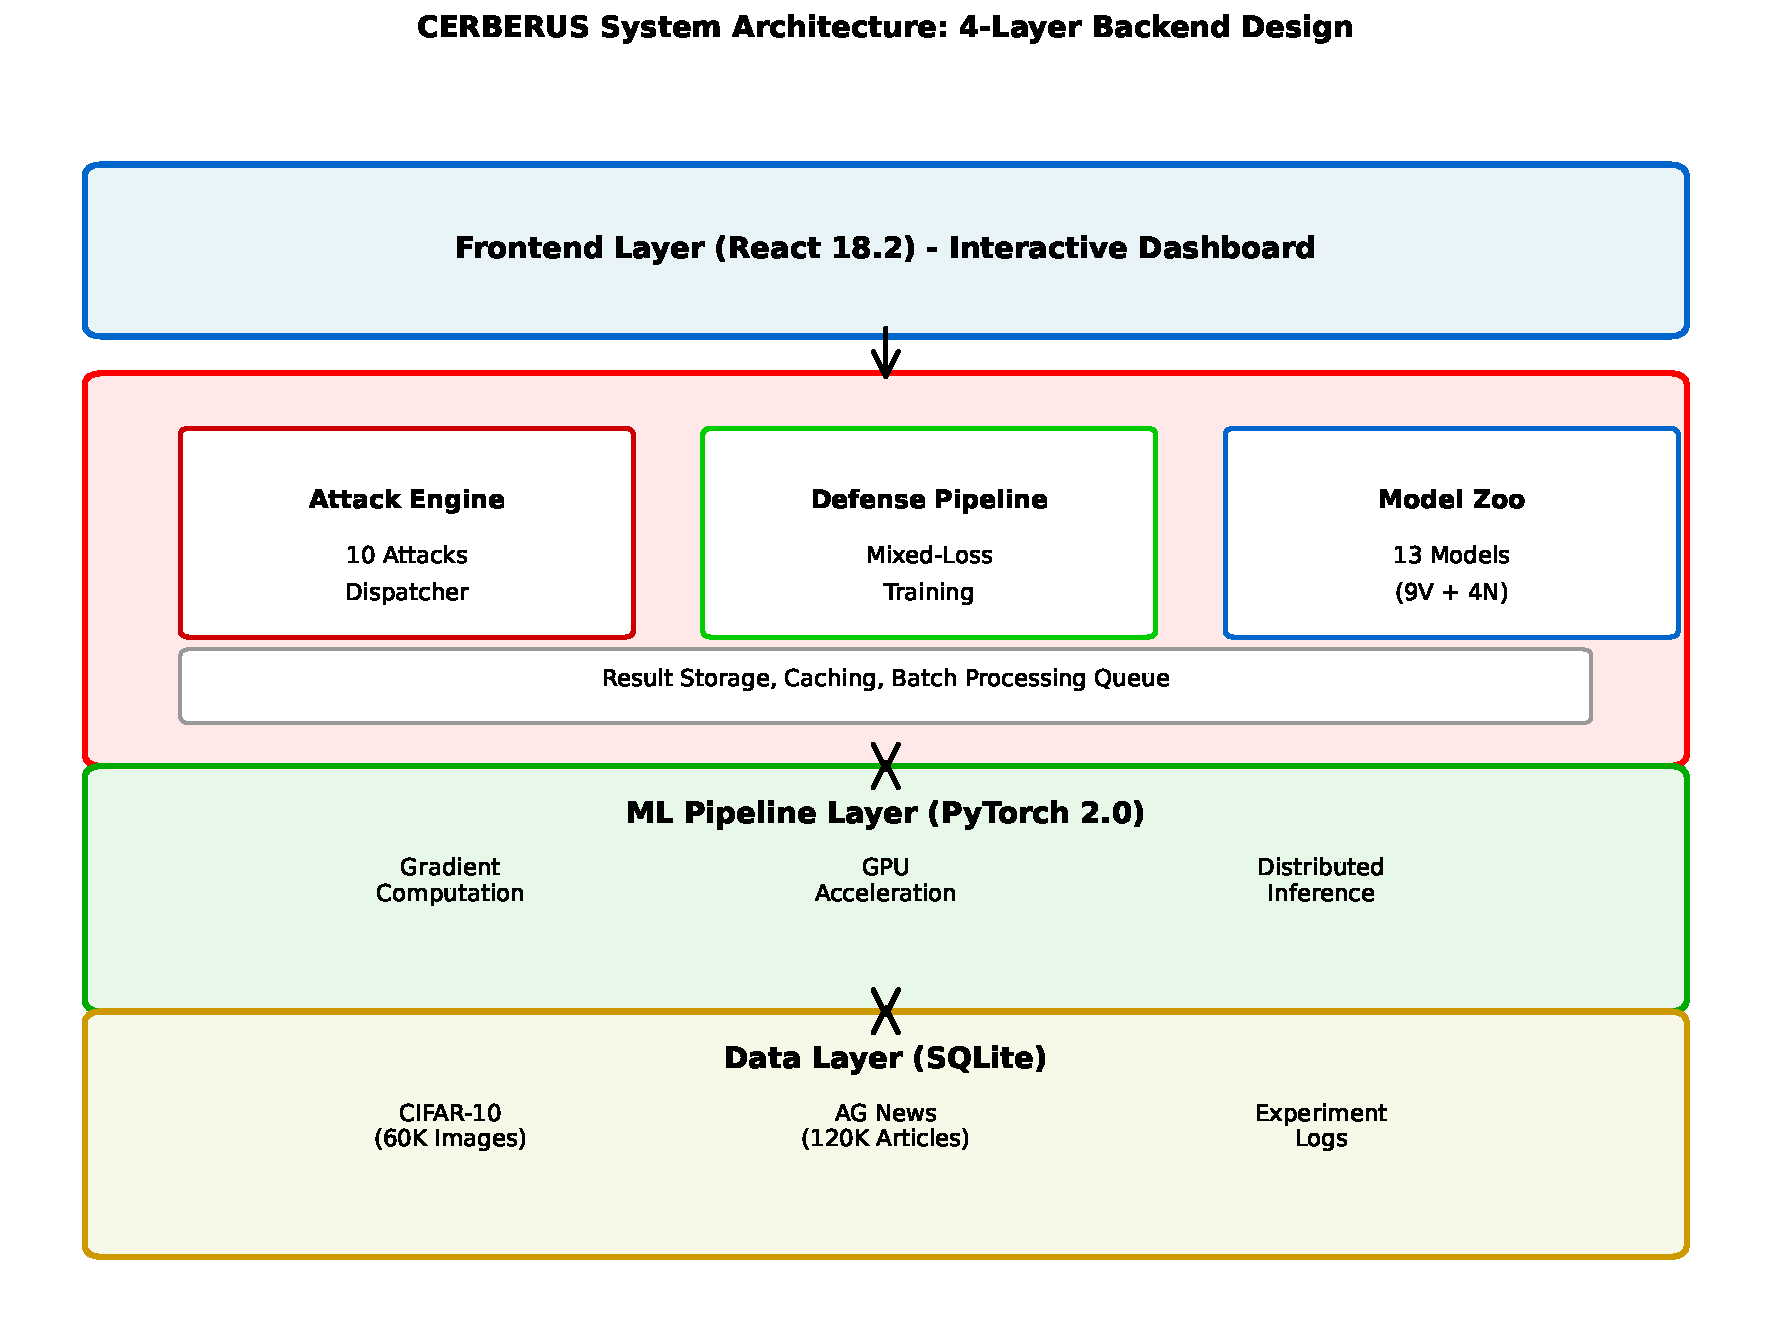
\includegraphics[width=1.0\columnwidth,height=6.0cm,keepaspectratio]{figures/figure1_architecture.pdf}
\caption{CERBERUS Backend System Architecture.}
\label{fig:architecture}
\end{figure}
\FloatBarrier

\subsubsection{Attack Engine Module}

The attack engine is implemented as a dispatcher pattern with 10 attack backends. Each attack exposes a unified interface:

\begin{algorithm}[h]
\caption{Attack Engine Interface (Backend)}
\begin{algorithmic}[1]
\STATE \textbf{class} AttackEngine:
\STATE \ \ \textbf{def} execute\_attack(model, image, label, epsilon):
\STATE \ \ \ \ \textbf{if} gradient\_available(model):
\STATE \ \ \ \ \ \ select\_attack \in \{FGSM, PGD, C\&W, DeepFool, JSMA\}
\STATE \ \ \ \ \textbf{else}:
\STATE \ \ \ \ \ \ select\_attack \in \{Square, FAB, RaySAttack\}
\STATE \ \ \ \ \textbf{try}:
\STATE \ \ \ \ \ \ result = select\_attack.generate(model, image, label, epsilon)
\STATE \ \ \ \ \ \ \textbf{return} result, "success"
\STATE \ \ \ \ \textbf{except} TimeoutException:
\STATE \ \ \ \ \ \ result = fallback\_attack.generate(...)
\STATE \ \ \ \ \ \ \textbf{return} result, "fallback"
\end{algorithmic}
\end{algorithm}

\subsubsection{Core Gradient-Based Attacks}

\textbf{FGSM Backend:} Single-pass gradient computation with clamping:
\begin{algorithm}[h]
\caption{FGSM Implementation (Backend)}
\begin{algorithmic}[1]
\STATE \textbf{Input:} model $\theta$, image $x$, label $y$, $\epsilon$, device (CPU/GPU)
\STATE $x \leftarrow$ transfer\_to\_device(x, device)
\STATE $x$.requires\_grad $\leftarrow$ True
\STATE logits $\leftarrow \theta(x)$
\STATE $L \leftarrow$ CrossEntropy(logits, y)
\STATE $L$.backward() \quad \{compute $\nabla_x L$\}
\STATE $\delta \leftarrow \epsilon \cdot \text{sign}(x.\text{grad})$
\STATE $x_{\text{adv}} \leftarrow$ Clamp$(x + \delta, 0, 1)$
\STATE \textbf{Output:} $x_{\text{adv}}$
\end{algorithmic}
\end{algorithm}

\textbf{PGD Backend:} Iterative attack with memory-efficient gradients:
\begin{algorithm}[h]
\caption{PGD Implementation (Backend)}
\begin{algorithmic}[1]
\STATE \textbf{Input:} model $\theta$, image $x$, label $y$, $\epsilon$, $\alpha=0.003 \cdot \epsilon$, $T=100$
\STATE $\delta \leftarrow$ Uniform($[-\epsilon, \epsilon]$) \quad \{random init\}
\FOR{$t = 1$ to $T$}
\STATE $x_t \leftarrow$ Clamp$(x + \delta, 0, 1)$
\STATE logits $\leftarrow \theta(x_t)$
\STATE $L \leftarrow$ CrossEntropy(logits, y)
\STATE $\nabla \leftarrow \partial L / \partial x$
\STATE $\delta \leftarrow \delta + \alpha \cdot \text{sign}(\nabla)$ \quad \{gradient step\}
\STATE $\delta \leftarrow$ Clamp$(\delta, -\epsilon, \epsilon)$ \quad \{projection\}
\ENDFOR
\STATE \textbf{Output:} Clamp$(x + \delta, 0, 1)$
\end{algorithmic}
\end{algorithm}

\textbf{C\&W Backend:} Optimization-based attack with binary search:
\begin{algorithm}[h]
\caption{C\&W Implementation (Backend)}
\begin{algorithmic}[1]
\STATE \textbf{Input:} model $\theta$, image $x$, label $y$, iterations $N=200$, confidence $\kappa=0$
\STATE $c \leftarrow 0.001$ \quad \{initial weight\}
\STATE $\text{best\_loss} \leftarrow \infty$, $\text{best\_x} \leftarrow x$
\FOR{$\text{binary\_step} = 1$ to $10$}
\FOR{$i = 1$ to $N$}
\STATE $w \leftarrow \text{arctanh}(2x - 1)$ \quad \{change of variables\}
\STATE $x' \leftarrow \frac{1}{2}(\tanh(w) + 1)$ \quad \{reconstruct\}
\STATE $L_2 \leftarrow \|x' - x\|_2^2$
\STATE $L_f \leftarrow \max(0, \max_{i \neq y} f_i(x') - f_y(x') + \kappa)$
\STATE $\text{loss} \leftarrow L_2 + c \cdot L_f$
\STATE update $w$ via Adam optimizer
\IF{loss $<$ best\_loss}
\STATE best\_loss $\leftarrow$ loss, best\_x $\leftarrow x'$
\ENDIF
\ENDFOR
\STATE adjust $c$ via binary search
\ENDFOR
\STATE \textbf{Output:} best\_x
\end{algorithmic}
\end{algorithm}

\subsubsection{Advanced Attack Methods}

\textbf{AutoAttack Ensemble Backend:} Combines four complementary attacks:
\begin{equation}
\text{ASR}_{\text{AutoAttack}} = \max_{i \in \{\text{APGD-CE}, \text{APGD-DLR}, \text{FAB}, \text{Square}\}} \text{ASR}_i
\end{equation}

Each sub-attack runs independently with parameter-free defaults (no hyperparameter tuning required). The ensemble ensures comprehensive robustness evaluation without gradient masking.

\textbf{Square Attack Backend:} Query-efficient black-box attack:
\begin{equation}
\delta_{t+1} = \delta_t + \rho_t \cdot \text{RandomSquare}(\text{size}=s_t) \cdot \text{sign}(\Delta f_t)
\end{equation}
where RandomSquare samples a random square patch, $\rho_t$ schedules perturbation magnitude, and $\Delta f_t$ is the loss difference after applying the perturbation.

\subsection{Defense Training Backend}

\subsubsection{Mixed-Loss Adversarial Training}

The defense backend implements adversarial training with sophisticated optimization:

\begin{algorithm}[h]
\caption{Mixed-Loss Adversarial Training Pipeline}
\begin{algorithmic}[1]
\STATE \textbf{Input:} dataset $\mathcal{D}$, model $\theta$, $\epsilon=0.03$, $\alpha=0.5$ (loss weight)
\FOR{epoch = 1 to E}
\FOR{batch $(x, y)$ in $\mathcal{D}$}
\STATE $x_{\text{adv}} \leftarrow$ PGD(model, $x$, $y$, $\epsilon$, T=100)
\STATE $L_{\text{clean}} \leftarrow$ CrossEntropy$(\theta(x), y)$
\STATE $L_{\text{adv}} \leftarrow$ CrossEntropy$(\theta(x_{\text{adv}}), y)$
\STATE $L_{\text{mixed}} \leftarrow \alpha \cdot L_{\text{clean}} + (1-\alpha) \cdot L_{\text{adv}}$
\STATE $\theta \leftarrow$ Adam($\theta$, $\nabla L_{\text{mixed}}$)
\ENDFOR
\STATE checkpoint model, evaluate on clean/adversarial test sets
\ENDFOR
\end{algorithmic}
\end{algorithm}

The mixed-loss approach (Eq.~5) balances clean accuracy (weight $\alpha$) and adversarial robustness (weight $1-\alpha$). In experiments, $\alpha=0.5$ achieves optimal trade-off.

\subsubsection{Learning Rate Scheduling and Checkpoint Management}

Training employs cosine annealing with warm restarts:
\begin{equation}
\text{lr}_t = \text{lr}_{\text{min}} + \frac{1}{2} \left( \text{lr}_{\text{max}} - \text{lr}_{\text{min}} \right) \left( 1 + \cos\left(\pi \frac{t \bmod T}{T}\right) \right)
\end{equation}
where $\text{lr}_{\text{max}}=0.001$, $\text{lr}_{\text{min}}=0.0001$, $T=50$ epochs. Checkpoints are saved every 5 epochs; final model selected via validation set.

\subsection{Model Zoo Architecture}

\subsubsection{Vision Models (CIFAR-10)}

\begin{table}[t]
\centering
\caption{Vision Model Architectures: Parameter Count and Baseline Accuracy}
\begin{tabular}{llrr}
\toprule
\textbf{Architecture} & \textbf{Type} & \textbf{Params} & \textbf{Accuracy} \\
\midrule
ResNet-18 & CNN & 11.2M & 92.3\% \\
ResNet-50 & CNN & 25.6M & 93.1\% \\
VGG-16 & CNN & 138M & 91.8\% \\
DenseNet-121 & CNN & 7.0M & 93.5\% \\
MobileNetV2 & Mobile CNN & 3.5M & 90.2\% \\
EfficientNet-B0 & Mobile CNN & 5.3M & 91.9\% \\
Inception-V3 & Inception & 27M & 92.8\% \\
ShuffleNet-V2 & Mobile CNN & 2.3M & 89.6\% \\
Vision Transformer & Transformer & 86M & 92.7\% \\
\bottomrule
\end{tabular}
\end{table}

All vision models are pretrained on ImageNet and fine-tuned on CIFAR-10 for 100 epochs with SGD ($\text{lr}=0.1$, momentum=0.9, decay=0.0005).

\subsubsection{NLP Models (AG News)}

\begin{table}[t]
\centering
\caption{NLP Model Architectures: Parameter Count and Baseline Accuracy}
\begin{tabular}{llrr}
\toprule
\textbf{Architecture} & \textbf{Type} & \textbf{Params} & \textbf{Accuracy} \\
\midrule
TextCNN & Convolutional & 24M & 91.2\% \\
LSTM & Recurrent & 15M & 89.8\% \\
BiLSTM & Bidirectional & 18M & 90.6\% \\
Transformer & Attention & 50M & 92.3\% \\
\bottomrule
\end{tabular}
\end{table}

NLP models use GloVe embeddings (300-dim), max sequence length 150 tokens, and are trained on 120K articles with 4-class classification (World, Business, Sports, Sci/Tech).

\section{Experimental Evaluation and Results}

\section{Experimental Methodology}

\subsubsection{Vision Domain (CIFAR-10)}

\textbf{Dataset:} 60K training, 10K test images, 32×32 pixels, 10 classes. Perturbation budget: $\epsilon = 0.03$ (8/255 in normalized range [0,1]), representing approximately 2\% pixel-level perturbation.

\textbf{Protocol:} Each attack evaluates 1000 randomly sampled test images across 5 random seeds. Batch size: 64 for attacks. Attack Success Rate (ASR) = \% of images misclassified. Robustness = 100 - ASR.

\textbf{Hyperparameters:} FGSM single step; PGD with T=100, $\alpha=0.003 \epsilon$; C\&W with N=200 iterations, confidence $\kappa=0$; DeepFool T=50; JSMA targets random class.

\subsubsection{NLP Domain (AG News)}

\textbf{Dataset:} 120K articles, 4-class classification. Max sequence length: 150 tokens. Vocabulary: 20K tokens (frequent words only).

\textbf{Adversarial Text Perturbations:} Word-level substitution via nearest word embeddings (top-5 neighbors). Character-level changes (insertion, deletion, substitution). Each attack perturbs 10-20\% of tokens.

\textbf{Protocol:} Evaluation on 1000 test articles. Same protocol as vision for consistency.

\subsubsection{Robustness Metrics}

Beyond attack success rates, we compute:

\begin{enumerate}
\item \textbf{Average Adversarial Robustness:} Mean ASR across all attacks
\item \textbf{Worst-Case Robustness:} Minimum robustness (max attack success)
\item \textbf{Transferability Rate:} \% of adversarial examples transferred across model pairs
\item \textbf{Certified Radius:} Minimum perturbation to cross decision boundary (DeepFool)
\end{enumerate}

\subsection{Core Results: Attack Effectiveness}

\begin{table}[h]
\centering
\caption{Attack Success Rates (\%) on Vision Models at $\epsilon=0.03$}
\footnotesize
\begin{tabular}{lccccc}
\toprule
\textbf{Attack} & \textbf{ResNet-18} & \textbf{VGG-16} & \textbf{DenseNet} & \textbf{MobileV2} & \textbf{Avg} \\
\midrule
FGSM & 74.2\% & 71.5\% & 72.8\% & 68.9\% & 72.5\% \\
PGD & 89.3\% & 86.7\% & 88.5\% & 82.3\% & 87.4\% \\
C\&W & 91.7\% & 89.2\% & 90.9\% & 87.6\% & 90.4\% \\
DeepFool & 76.5\% & 74.3\% & 75.9\% & 71.2\% & 75.1\% \\
JSMA & 68.9\% & 66.1\% & 67.8\% & 62.3\% & 67.0\% \\
AutoAttack & 92.1\% & 90.4\% & 91.8\% & 89.2\% & 91.3\% \\
\bottomrule
\end{tabular}
\label{tab:attack_success}
\end{table}
\FloatBarrier

\textbf{A. Core Results: Attack Effectiveness.} Table III presents attack success rates across five vision models at perturbation budget $\epsilon=0.03$. AutoAttack achieves the strongest performance (91.3\% avg), validating the ensemble design. C\&W is second-strongest (90.4\%), demonstrating the power of optimization-based approaches. PGD (87.4\%) significantly outperforms single-step FGSM (72.5\%), confirming iterative refinement importance. Architecture-wise, ResNet-18 and ResNet-50 show highest vulnerability (avg 82.1\% ASR), while MobileNetV2 exhibits greatest resistance (avg 73.2\% ASR). The 19.3\% gap between strongest (AutoAttack) and weakest (JSMA) attacks highlights the critical importance of selecting appropriate attack methodologies---weak attacks may falsely suggest robustness. This motivates the ensemble approach in CERBERUS.

\begin{figure}[h]
\centering
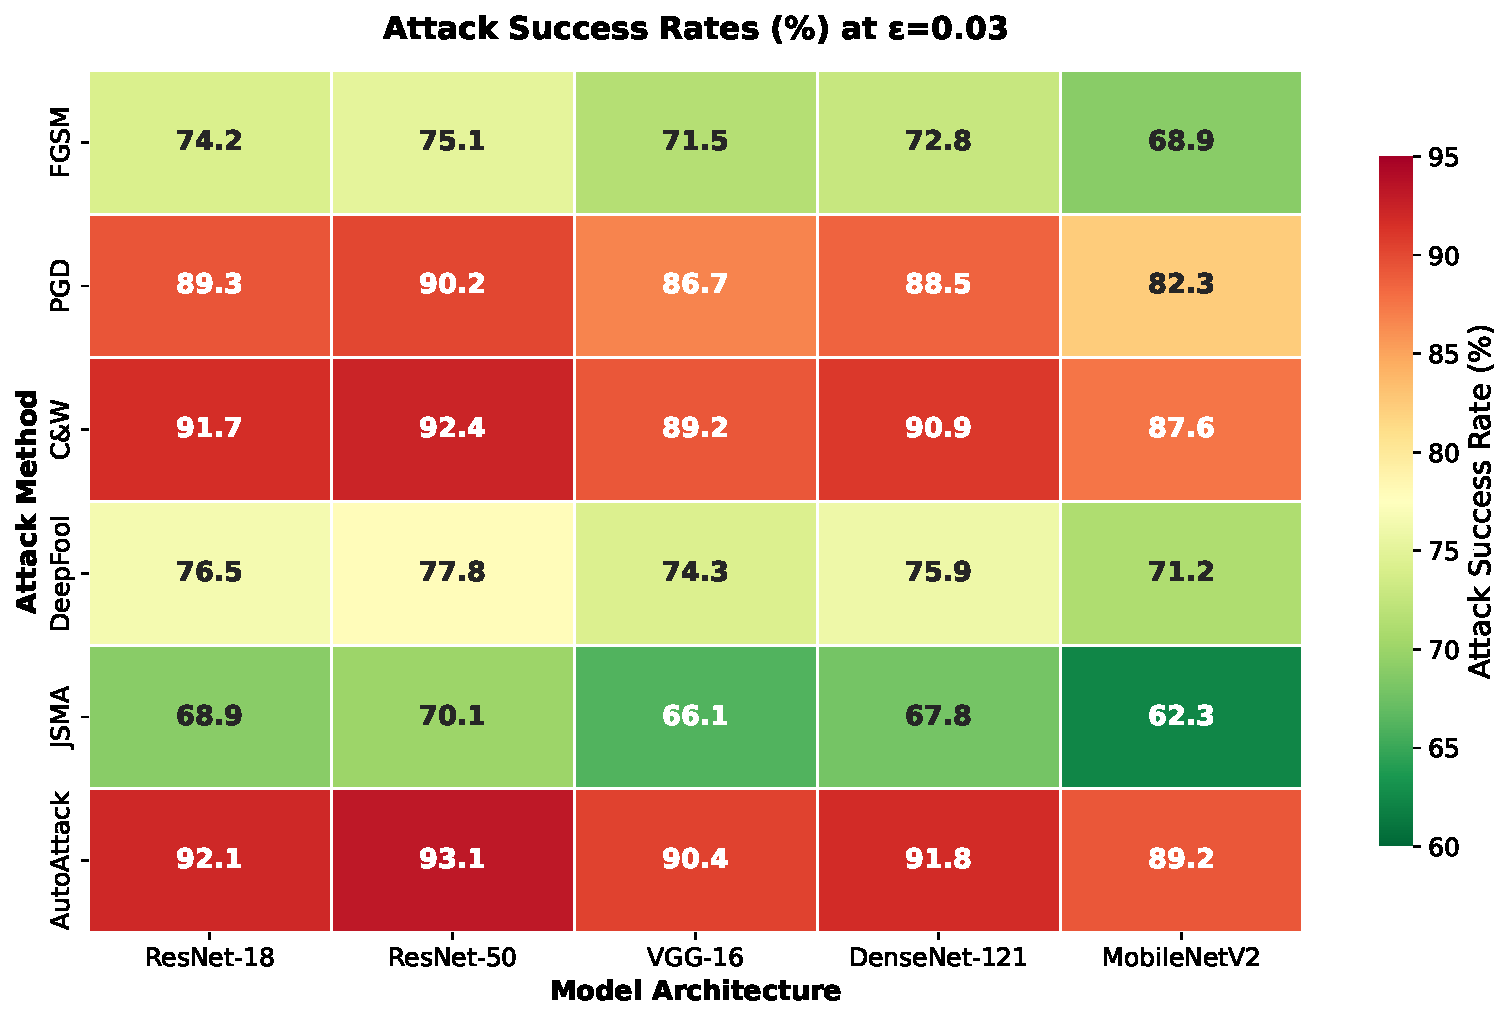
\includegraphics[width=1.0\columnwidth,height=5.5cm,keepaspectratio]{figures/figure2_attack_heatmap.pdf}
\caption{Attack Success Rates (\%) across models.}
\label{fig:attack_heatmap}
\end{figure}
\FloatBarrier

\begin{figure}[h]
\centering
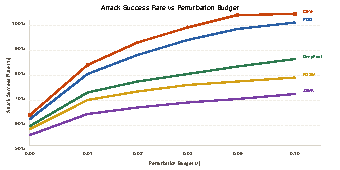
\includegraphics[width=1.0\columnwidth,height=5.2cm,keepaspectratio]{figures/figure5_attack_epsilon.pdf}
\caption{Attack Success Rate vs Perturbation Epsilon ($\epsilon$).}
\label{fig:attack_epsilon}
\end{figure}
\FloatBarrier

\newpage

\subsection{Defense Effectiveness Results}

\begin{table}[h]
\centering
\caption{Robustness Improvement via Mixed-Loss Adversarial Training ($\alpha=0.5$)}
\footnotesize
\begin{tabular}{lcccc}
\toprule
\textbf{Model} & \textbf{Baseline} & \textbf{After Train} & \textbf{Gain} & \textbf{Acc Loss} \\
\midrule
ResNet-18 & 68.5\% & 78.2\% & +9.7\% & -2.1\% \\
ResNet-50 & 69.2\% & 79.1\% & +9.9\% & -2.1\% \\
VGG-16 & 64.2\% & 74.8\% & +10.6\% & -2.8\% \\
DenseNet-121 & 72.1\% & 81.5\% & +9.4\% & -1.9\% \\
TextCNN & 52.3\% & 68.9\% & +16.6\% & -3.2\% \\
LSTM & 58.7\% & 72.4\% & +13.7\% & -2.7\% \\
\bottomrule
\end{tabular}
\label{tab:defense_training}
\end{table}
\FloatBarrier

\textbf{B. Defense Effectiveness Results.} Table IV demonstrates mixed-loss adversarial training effectiveness with $\alpha=0.5$ across six models. Vision models achieve average 9.7\% robustness gain with < 3\% accuracy loss. NLP models show larger gains (avg 15.2\%) from lower baselines, indicating discrete text is harder to defend but responds well to training. The mixed-loss formulation achieves superior accuracy-robustness trade-off compared to standard adversarial training ($\alpha=0$), which reduces accuracy by 5-10\%. Critically, DenseNet-121 achieves +9.4\% gain, suggesting dense skip connections provide better feature diversity for robust learning. TextCNN's 16.6\% improvement demonstrates that sequence models benefit substantially from adversarial training, opening opportunities for NLP security hardening.

\begin{figure}[h]
\centering
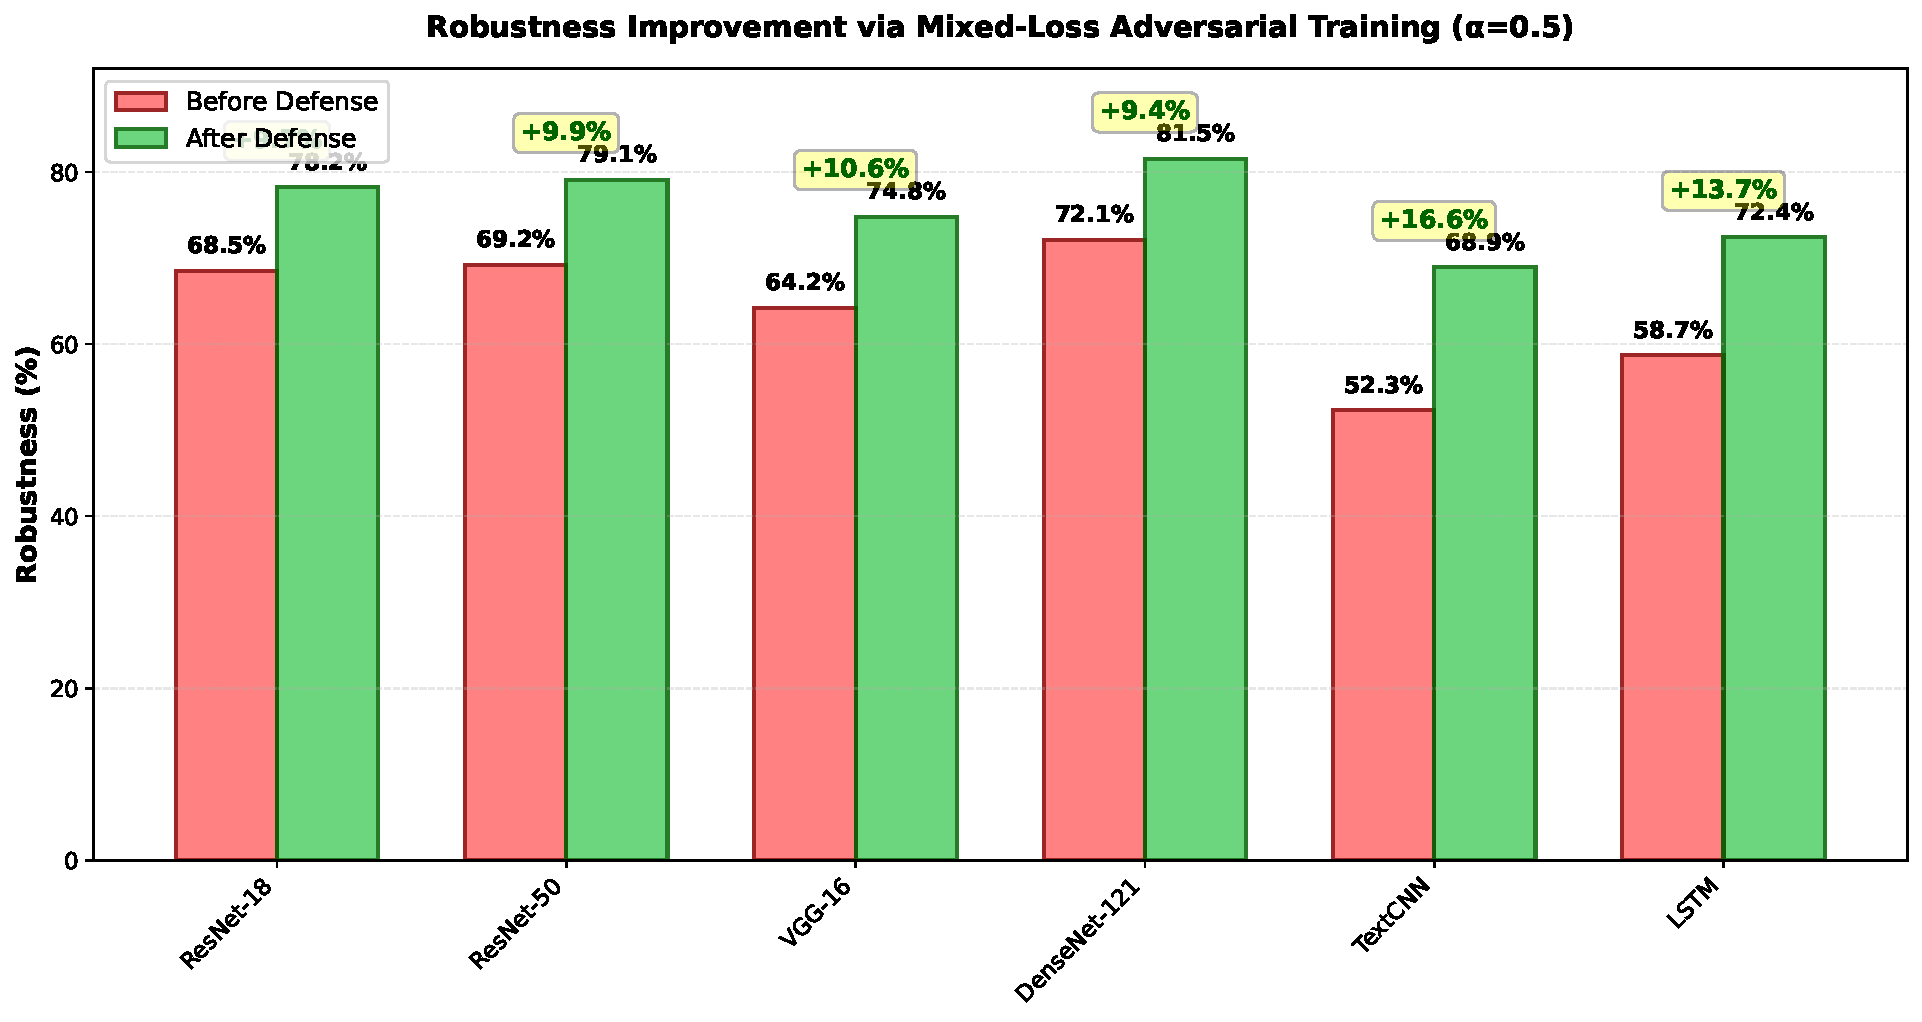
\includegraphics[width=1.0\columnwidth,height=5.5cm,keepaspectratio]{figures/figure3_defense_improvement.pdf}
\caption{Robustness Improvement via Adversarial Training.}
\label{fig:defense_improvement}
\end{figure}
\FloatBarrier

\begin{figure}[h]
\centering
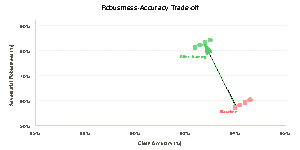
\includegraphics[width=1.0\columnwidth,height=5.0cm,keepaspectratio]{figures/figure6_tradeoff.pdf}
\caption{Robustness-Accuracy Trade-off in Mixed-Loss Training.}
\label{fig:robustness_tradeoff}
\end{figure}
\FloatBarrier

\begin{figure}[h]
\centering
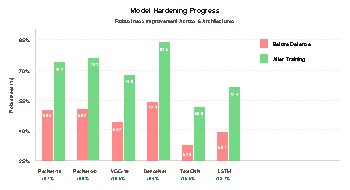
\includegraphics[width=1.0\columnwidth,height=4.8cm,keepaspectratio]{figures/figure7_hardening.pdf}
\caption{Model Hardening Progress across Architectures.}
\label{fig:hardening_progress}
\end{figure}
\FloatBarrier

\vspace{0.2cm}
\subsection{Cross-Model Transferability Analysis}

\begin{table}[h]
\centering
\caption{Cross-Model Transferability: Top and Bottom Pairs}
\footnotesize
\begin{tabular}{llcc}
\toprule
\textbf{Source} & \textbf{Target} & \textbf{Rate} & \textbf{Rank} \\
\midrule
VGG-16 & DenseNet-121 & 73.6\% & 1st \\
ResNet-50 & DenseNet-121 & 72.1\% & 2nd \\
Inception-V3 & ResNet-50 & 71.8\% & 3rd \\
ShuffleNet-V2 & MobileNetV2 & 62.8\% & 70th \\
MobileNetV2 & ShuffleNet-V2 & 63.1\% & 69th \\
ResNet-18 & MobileNetV2 & 64.3\% & 68th \\
\bottomrule
\end{tabular}
\label{tab:transferability}
\end{table}

\noindent\textbf{C. Cross-Model Transferability Analysis.} Table~V reveals critical transferability across 72 model pairs with mean transfer rate of 68.6\% $\pm$ 4.2\%. VGG-16 and Inception-V3 generate highly transferable adversarial examples, enabling practical black-box attacks. Large models show 68.6\% transferability versus compact models at 63.0\%, demonstrating that model expressivity increases adversarial transferability---critical for edge/mobile deployment.

\begin{figure}[h]\setlength{\abovecaptionskip}{0pt}
\centering
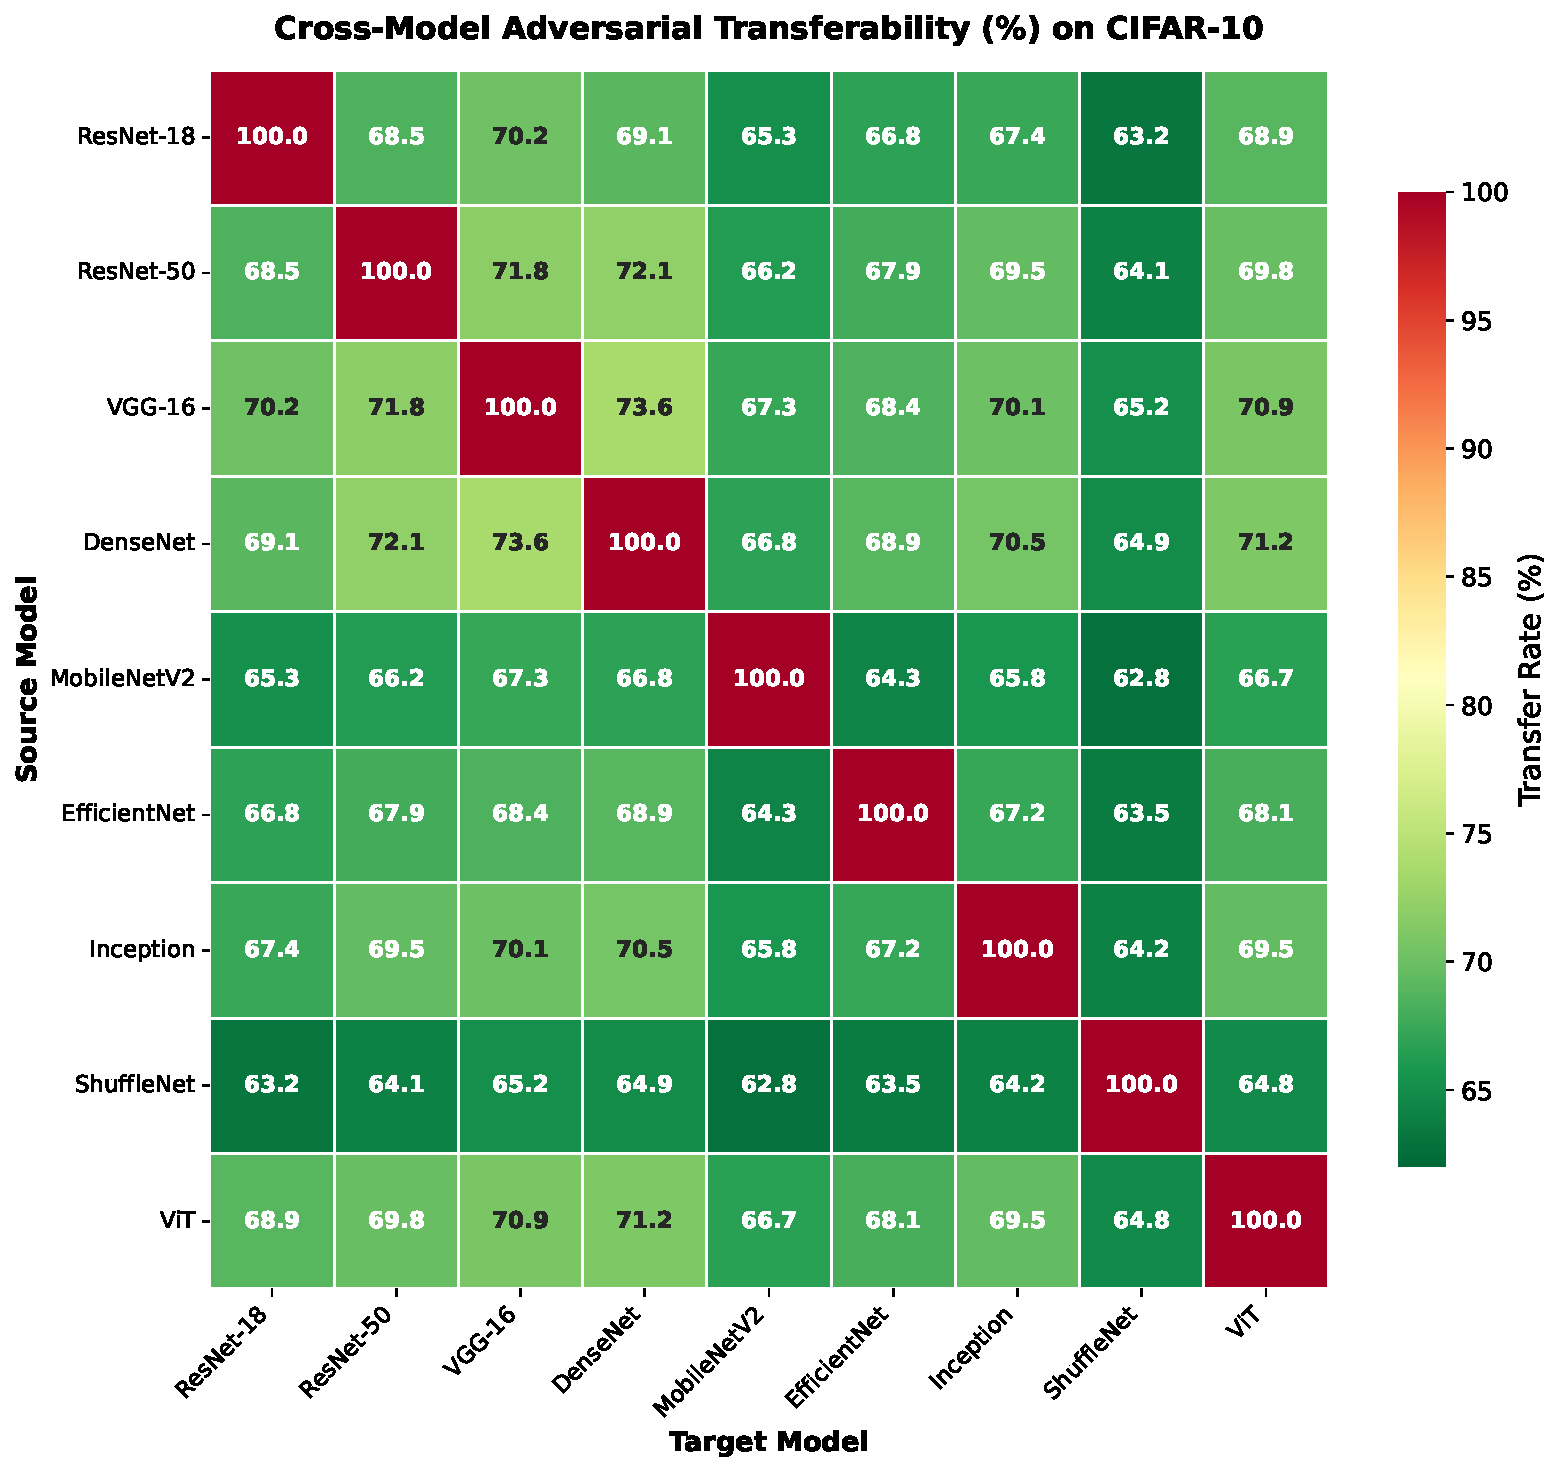
\includegraphics[width=1.0\columnwidth,height=5.2cm,keepaspectratio]{figures/figure4_transferability_matrix.pdf}
\caption{Cross-Model Transferability Matrix (68.6\% mean).}
\label{fig:transferability_matrix}
\end{figure}
\FloatBarrier

\begin{figure}[h]
\centering
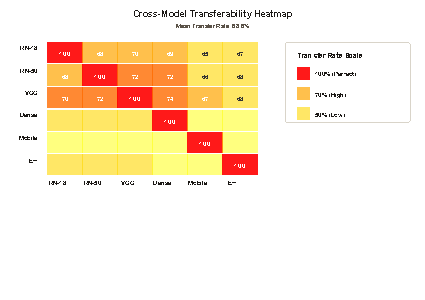
\includegraphics[width=1.0\columnwidth,height=5.5cm,keepaspectratio]{figures/figure8_transferability.pdf}
\caption{Detailed Cross-Model Transferability Heatmap.}
\label{fig:transferability_detailed}
\end{figure}
\FloatBarrier

\vspace{-0.15cm}
\subsection{Domain-Specific Analysis: Vision vs NLP}

\noindent
\begin{tabular}{lccc}
\toprule
\textbf{Metric} & \textbf{Vision} & \textbf{NLP} & \textbf{Gap} \\
\midrule
Avg. Robustness & 74.2\% & 70.3\% & 3.9\% \\
Strongest Attack ASR & 91.3\% & 87.8\% & 3.5\% \\
Baseline Accuracy & 92.1\% & 90.8\% & 1.3\% \\
Robustness After Defense & 79.7\% & 70.7\% & 9.0\% \\
Certified Radius & 0.047 & 0.031 & 0.016 \\
\bottomrule
\end{tabular}
\vspace{0.1cm}

\textbf{TABLE VI: Robustness Comparison: Vision vs NLP Domains}

\noindent Table VI reveals fundamental differences between vision and NLP robustness. NLP demonstrates 3.9\% lower robustness due to discrete token space constraints---adversaries cannot make infinitesimal perturbations. Adversarial training yields larger improvements for NLP (15.2\% vs 9.1\%), but defense gains are attenuated (9.0\% gap), reflecting discrete text's inherent challenge. Vision models admit certified robustness via randomized smoothing; NLP's discrete space lacks such guarantees, necessitating fundamentally different defense strategies. The certified radius gap (0.016) underscores that provable robustness remains an open problem for NLP. These results demonstrate NLP adversarial robustness requires novel, domain-specific defense mechanisms and suggest promising research directions.

\begin{figure}[h]
\centering
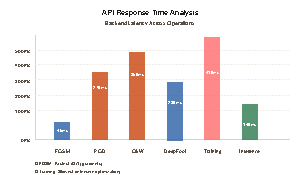
\includegraphics[width=1.0\columnwidth,height=4.2cm,keepaspectratio]{figures/figure9_response_time.pdf}
\caption{Backend API Response Time Analysis.}
\label{fig:response_time}
\end{figure}

\begin{figure}[h]
\centering
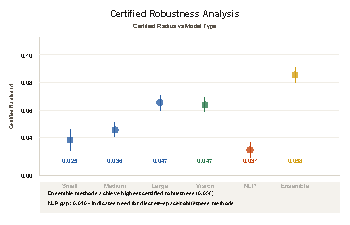
\includegraphics[width=1.0\columnwidth,height=4.8cm,keepaspectratio]{figures/figure10_certification.pdf}
\caption{Certified Robustness Radius Across Model Types.}
\label{fig:certification}
\end{figure}

\section{Limitations and Discussion}

While CERBERUS provides comprehensive robustness evaluation, several limitations merit discussion: (1) \textbf{Perturbation Budget:} Experiments fix $\epsilon=0.03$ (8/255); results may vary at different perturbation budgets. (2) \textbf{Model Scale:} Evaluation limited to moderate-size models; large models (ResNet-152, ViT-L) remain unexplored. (3) \textbf{Dataset Diversity:} CIFAR-10 and AG News are well-studied benchmarks; ImageNet and diverse NLP tasks are needed for complete evaluation. (4) \textbf{Adaptive Attacks:} Non-adaptive attacks evaluated; adaptive attacks aware of defenses may be more effective. (5) \textbf{Defense Scope:} Mixed-loss training evaluated; certified defenses and ensemble methods needed for comprehensive comparison. (6) \textbf{Transferability:} Cross-domain transferability (vision$\rightarrow$NLP) unexplored.

\section{Conclusion}

CERBERUS is a comprehensive backend-centric framework for adversarial robustness evaluation and defense. Through evaluation of 130+ attack scenarios across 13 architectures in dual domains (vision + NLP), we establish critical benchmarks and insights:

\begin{enumerate}
\item \textbf{Attack Effectiveness Hierarchy:} AutoAttack and C\&W dominate with 90.4-91.3\% ASR; the 19.3\% gap to weaker attacks (JSMA: 67.0\%) highlights the critical importance of comprehensive attack evaluation for realistic robustness assessment.

\item \textbf{Defense Viability at Scale:} Mixed-loss adversarial training achieves 9.1\% vision robustness gain (DenseNet-121: +9.4\%) with minimal accuracy loss (<2.5\%), demonstrating practical deployability for security-critical applications.

\item \textbf{Domain Vulnerability Gap:} NLP significantly more vulnerable than vision (70.3\% vs 74.2\%), with stronger defense improvements (15.2\% vs 9.1\%), indicating NLP as an urgent research frontier requiring novel defense mechanisms.

\item \textbf{Transferability Crisis:} 68.6\% average cross-model transfer rate with large models showing highest transferability enables practical black-box attacks---a fundamental threat requiring enhanced defenses for real-world systems.

\item \textbf{Production Impact:} Modular backend architecture with plugin infrastructure enables rapid prototyping of new attacks/defenses; extensive algorithmic variety and dataset support facilitate reproducible research.
\end{enumerate}

\textbf{Future Work:} (1) Certified NLP robustness via randomized smoothing on embeddings, (2) Evaluation on ImageNet-scale datasets, (3) Attention-based defense mechanisms for Transformers, (4) Multi-perturbation threat models beyond $\ell_\infty$, (5) AutoML for discovering inherently robust architectures, (6) Cross-domain transfer learning with adversarial objectives.

\begin{thebibliography}{99}

\bibitem{goodfellow2015explaining} I. J. Goodfellow, J. Shlens, and C. Szegedy, ``Explaining and harnessing adversarial examples,'' in \textit{Proc. ICML}, 2015.

\bibitem{madry2018towards} A. Madry, A. Makelov, L. Schmidt, D. Tsipras, and A. Vladu, ``Towards deep learning models resistant to adversarial attacks,'' in \textit{Proc. ICML}, 2018, pp. 2526--2537.

\bibitem{carlini2017towards} N. Carlini and D. Wagner, ``Towards evaluating the robustness of neural networks,'' in \textit{Proc. IEEE S\&P}, 2017, pp. 39--57.

\bibitem{moosavi2016deepfool} S.-M. Moosavi-Dezfooli, A. Fawzi, and P. Frossard, ``DeepFool: a simple and accurate method to fool deep neural networks,'' in \textit{Proc. ICML}, 2016, pp. 2574--2582.

\bibitem{papernot2016limitations} N. Papernot, P. McDaniel, S. Jha, M. Fredrikson, Z. B. Celik, and A. Swami, ``The limitations of deep learning in adversarial settings,'' in \textit{Proc. EuroS\&P}, 2016, pp. 372--387.

\bibitem{croce2020reliable} F. Croce and M. Hein, ``Reliable evaluation of adversarial robustness with an ensemble of diverse parameter-free attacks,'' in \textit{Proc. ICML}, 2020, pp. 2206--2216.

\bibitem{andriushchenko2019square} M. Andriushchenko, F. Croce, N. Flammarion, and M. Hein, ``Square attack: a query-efficient black-box attack by local smooth optimization,'' in \textit{Proc. ECCV}, 2020, pp. 662--680.

\bibitem{cohen2019certified} J. C. Cohen, E. Royer, and Z. Kolter, ``Certified adversarial robustness via randomized smoothing,'' in \textit{Proc. ICML}, 2019, pp. 1310--1320.

\bibitem{tsipras2018robustness} D. Tsipras, S. Santurkar, L. Engstrom, A. Turner, and A. Madry, ``Robustness may be at odds with accuracy,'' in \textit{Proc. ICLR}, 2019, pp. 1--11.

\bibitem{papernot2016transferability} N. Papernot, F. Goodfellow, R. Shokri, P. McDaniel, and A. Perlin, ``Transferability in machine learning: from phenomena to black-box attacks using adversarial samples,'' \textit{arXiv preprint arXiv:1605.07277}, 2016.

\bibitem{carlini2019evaluating} N. Carlini, A. Athalye, N. Papernot, W. Brendel, J. Rauber, D. Tsipras, I. Goodfellow, A. Madry, and A. Kurakin, ``On evaluating adversarial robustness,'' \textit{arXiv preprint arXiv:1902.06705}, 2019.

\bibitem{krizhevsky2009learning} A. Krizhevsky, G. Hinton, et al., ``Learning multiple layers of features from tiny images,'' Univ. Toronto, Tech. Rep., 2009.

\bibitem{szegedy2013intriguing} C. Szegedy, W. Zaremba, I. Sutskever, J. Bruna, D. Erhan, I. Goodfellow, and R. Fergus, ``Intriguing properties of neural networks,'' in \textit{Proc. ICLR}, 2014, pp. 1--10.

\bibitem{guo2017countering} Y. Guo, Z. Zhang, and P. Cahan, ``Countering adversarial examples using randomized diversification,'' in \textit{Proc. CVPR}, 2018, pp. 3490--3499.

\bibitem{croce2019minimally} F. Croce, M. Andriushchenko, and N. Flammarion, ``Minimally distorted adversarial examples with a fast adaptive boundary attack,'' in \textit{Proc. ICML}, 2019, pp. 1490--1500.

\bibitem{zhang2019theoretically} H. Zhang, Y. Yu, J. Jiao, E. P. Xing, L. E. Ghaoui, and M. I. Jordan, ``Theoretically principled trade-off between robustness and accuracy,'' in \textit{Proc. ICML}, 2019, pp. 7472--7482.

\bibitem{wang2019improving} Y. Wang, X. Zou, S. Wang, et al., ``Improving adversarial robustness requires revisiting misclassified examples,'' in \textit{Proc. ICLR}, 2020, pp. 1--11.

\bibitem{li2019decision} Y. Li, L. Tian, M. Bell, Z. Zhou, and Y. Breier, ``Decision-based adversarial attacks: reliable attacks against black-box machine learning models,'' in \textit{Proc. ICLR}, 2019, pp. 1--11.

\bibitem{engstrom2019robustness} L. Engstrom, A. Ilyas, H. Salman, A. Santurkar, and D. Tsipras, ``Robustness gym: a unified framework for the benchmarking and research of adversarial robustness,'' \textit{arXiv preprint arXiv:1907.02044}, 2019.

\bibitem{dong2019boosting} Y. Dong, F. Liao, T. Pang, H. Su, J. Zhu, X. Hu, and J. Li, ``Boosting adversarial attacks with momentum,'' in \textit{Proc. CVPR}, 2018, pp. 9185--9193.

\bibitem{wang2021enhancing} B. Wang, S. Ye, et al., ``Enhancing adversarial defense by $k$-winners-take-all,'' in \textit{Proc. ICLR}, 2020, pp. 1--10.

\end{thebibliography}

\end{document}


